\documentclass[border=2mm]{standalone}
\usepackage[usenames,dvipsnames]{xcolor}
\usepackage{tikz}
\usetikzlibrary{shapes.multipart}
%\newcommand{\cc}{c\nolinebreak\hspace{-.05em}\raisebox{.2ex}{\tiny\bf +}\nolinebreak\hspace{-.10em}\raisebox{.2ex}{\tiny\bf +}}

\newcommand{\vardonut}[1]{
\newcounter{num}
\foreach \content/\size/\colour in {#1}
    \stepcounter{num};
\foreach \content/\size/\colour [count=\i] in {#1}{
    \draw[white,very thick,top color=\colour!80!black, bottom color=\colour, shading angle={-90+360/\thenum/2+(\i-1)*360/\thenum}] 
    ({2*cos((\i-1)*360/\thenum)},{2*sin((\i-1)*360/\thenum)}) arc[radius = 2, start angle={(\i-1)*360/\thenum}, delta angle=360/\thenum] --
    ({(2+\size)*cos(\i*360/\thenum)},{(2+\size)*sin(\i*360/\thenum)}) arc[radius = {2+\size}, start angle={\i*360/\thenum}, delta angle=-360/\thenum] -- 
    cycle;
    \node[Black,font=\Large,rotate=(\i-1)*360/\thenum+360/\thenum/2,text
    width=0.8*\size cm,align=left,anchor=west] at
    ({(\i-1)*360/\thenum+360/\thenum/2}:{2}) {\content  };
 }
}

\begin{document}
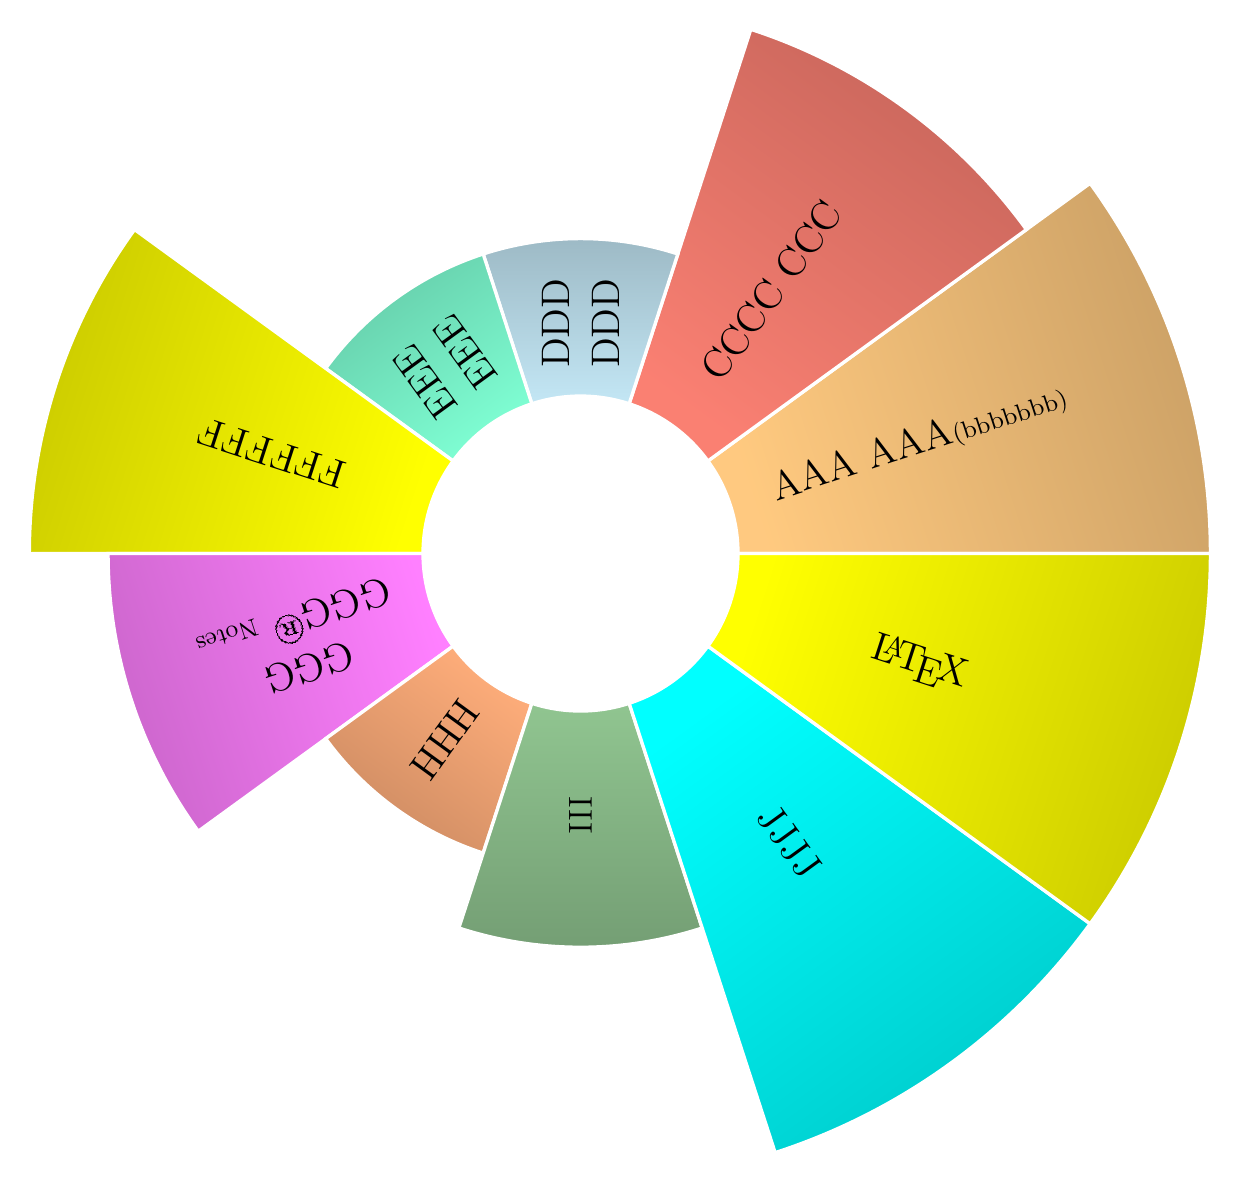
\begin{tikzpicture}[every text node part/.style={align=center}]
    \vardonut{AAA AAA\small({bbbbbbb})/6/YellowOrange!50!, CCCC CCC/5/Salmon,
    DDD DDD/2/SkyBlue!50!, EEE EEE/2/Aquamarine,FFFFFF/5/Yellow, GGG GGG\textsuperscript{\textregistered} \small{Notes}/4/Magenta!50!, HHH/2/Apricot,  \large{III }/3/ForestGreen!50!,JJJJ/6/Cyan,\LaTeX/6/Yellow}

\end{tikzpicture}
\end{document}    

